\vspace{-3pt}
\section{Introduction}
\label{sec:introduction}

%\begin{figure}[h]
%	\centering
%	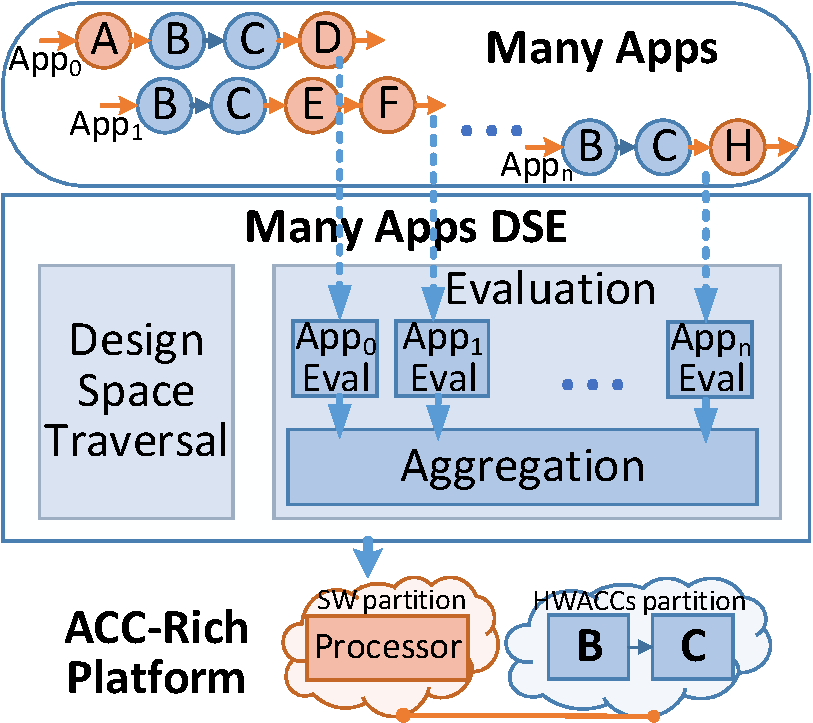
\includegraphics[width=.5\linewidth]{fig/MAARflow.pdf}
%	\caption{Promising Many Apps ACC-Rich Platform}
%	\label{fig:domainDSE}
%\end{figure}

%Tips: Mention Embedded or edge computing.

%(One common platform benefit)
Stream computing is essential in many fields, e.g. video analytics, software-defined ration, and radar. However, they faces area and power limitations, especially in edge computing. 
Using heterogeneous ACC-rich platforms~\cite{melpignano2012platform} that combine general-purpose processor(s) (SW) and custom ACCs (HW) is the primary approach for efficient, high-performance stream computing.
Designing one platform for each application is not economical as the non-recurring engineering (NRE) cost.
\newtext{
There is a potential using one unified platform with the same set of ACCs to benefit a set of applications, since streaming applications within the same field always sharing similar functionalities and structures.
}
%For example, in \figref{fig:domainDSE}, a set of applications sharing B-C kernels benefit from a platform with B-C ACCs.
%Designing a unified platform supporting many applications saves the prohibitively non-recurring engineering (NRE) cost compared with application-specific dedicated platforms designs.

%(Targeting Area: Heterogeneous Apps + Many ACCs Arch)
Creating a unified platform for a set of applications manually is already very hard for applications with homogeneous, repeated computation patterns, such as employed in Deep Convolutional Neural Networks\cite{chen2018eyeriss}. 
It becomes intractable for applications such as computer vision and software-defined radio with a wide range of computationally intensive and functionality diverse heterogeneous kernels. 
A monolithic ACC is an efficient application-specific solution but is not suitable for many applications due to its low flexibility and diverse acceleration requirements from different applications.
\newtext{
Instead, using many composable ACCs (ACC-rich platform\cite{cong2014accelerator}) is a better approach supporting many applications. In ACC-rich platform, individual ACCs are less monolithic but smaller and configurable, and can be composed to accelerate different larger kernels (or even applications). As a result, the number of ACCs increases dramatically, the complexity of ACC allocation becomes high, and the design automation is needed.
}

%(Current Design Automation)
Current design automation mostly focuses on allocating one dedicated platform for one individual application. 
\newtext{
Directly allocating all dedicated ACCs from all applications will exceed platform area and power constraints.
Even if every application only nominates a small number of ACCs, the platform will end up to a large number of unique ACCs. E.g., Each of 40 OpenVX applications nominates only 2 ACCs, and it ends up to 25 unique ACCs). 
The design automation in the scope of many applications is needed.
}
Some many applications ideas can be extracted from Platform-Based Design (PBD)\cite{PBD}. PBD designs the interconnection for many applications based on statistical information, however, the ACC allocation is derived by engineering experiences. 
There is also much research about the mapping of different applications to an existing platform\cite{marwedel2011mapping}\cite{quan2013scenario}. However, automatically allocating one common platform for many applications has not received much attention. 


\begingroup
\setlength{\columnsep}{8pt}%
\begin{wrapfigure}{l}{0.5\linewidth}
	\vspace{-4pt}
	\begin{center}
		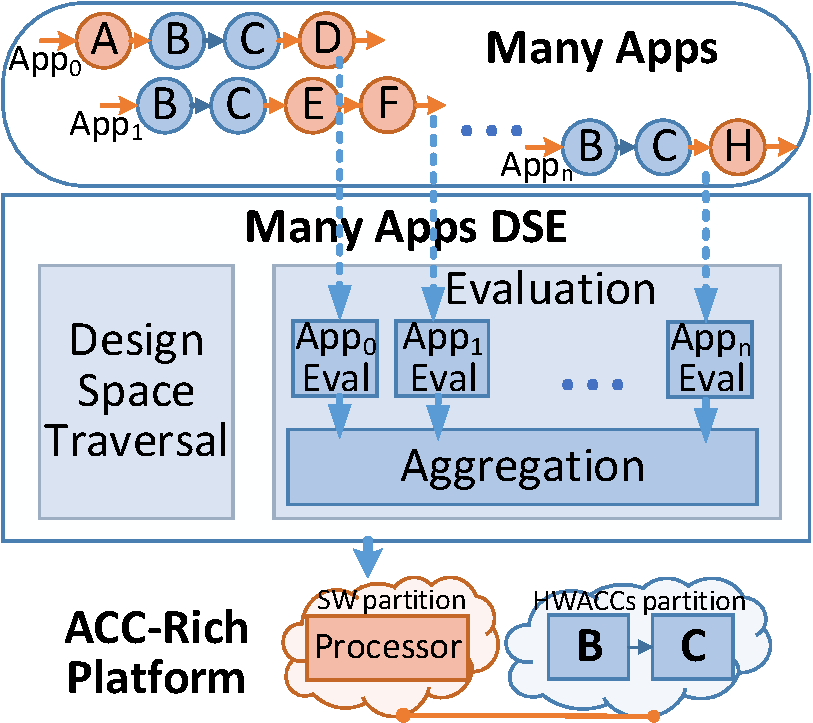
\includegraphics[width=\linewidth]{fig/MAARflow.pdf}
	\end{center}
	\vspace{-8pt}
	\caption{Unified Platform for Many Apps}
	\label{fig:domainDSE}
	\vspace{-4pt}
\end{wrapfigure}


%(Chanlleges)
\figref{fig:domainDSE} illustrates the general principles and challenges for ACC allocating one platform for many applications. The main challenges are traversal and evaluation.  
Due to targeting to multiple applications, the design space of platform allocation is significantly larger than single application design, and an efficient traversal is necessary.
Furthermore, the evaluation for many applications needs to be fair across applications to provide an aggregate metrics. Current evaluation primarily focuses on the effects of the platform on one application in isolation. When moving to a set of applications, the simple average sum of all application performances is unfair.

\endgroup





%Using heterogeneous ACC-rich platforms~\cite{melpignano2012platform} that combine general-purpose processor(s) (SW) and custom ACCs (HW) is the primary approach for efficient, high-performance stream computing.
%These platforms are typically designed targeting only a single application during allocation. Design Space Exploration (DSE) of one platform for each application is prohibitively expensive. In contrast to deep learning applications which often are computationally homogeneous and regular, such that a single monolithic accelerator can perform all linear algebraic computation required by deep learning algorithms, applications such as computer vision and software-defined radio demands a wide range of computationally intensive and functionality diverse heterogeneous accelerators (ACCs). The number of ACCs will increase dramatically, where individual ACCs are less monolithic but smaller and configurable. ACCs can be composed to accelerate larger kernels (or even applications).


%\figref{fig:domainDSE} shows an example of a platform using $B$-$C$ ACCs to efficiently support many applications, which share $B$ and $C$ kernels. 
%However, designing these platforms is a tremendous effort taking a vast amount of empiric knowledge into account. There is only little DSE methodology support for Many Applications ACC-Rich (MAAR) platforms because there is no existing evaluation to guide platform allocation for many applications. To feasibly allocate MAAR platforms, a MAAR DSE focusing on a set of applications, instead of individual applications in isolation, is needed.

%\begin{figure}[ht]
%  \centering
%  \begin{minipage}[t]{0.24\textwidth}
%    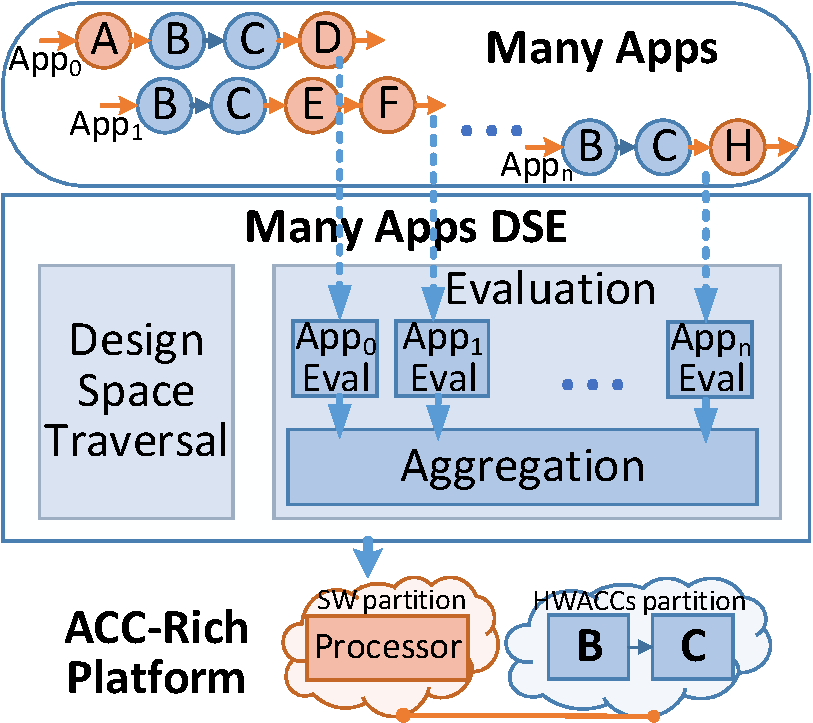
\includegraphics[width=.95\textwidth]{fig/MAARflow.pdf}
%    \caption{Promising Many Apps ACC-Rich Platform}
%    \label{fig:domainDSE}
%  \end{minipage}%
%  \hfill
%  \begin{minipage}[t]{0.23\textwidth}
%    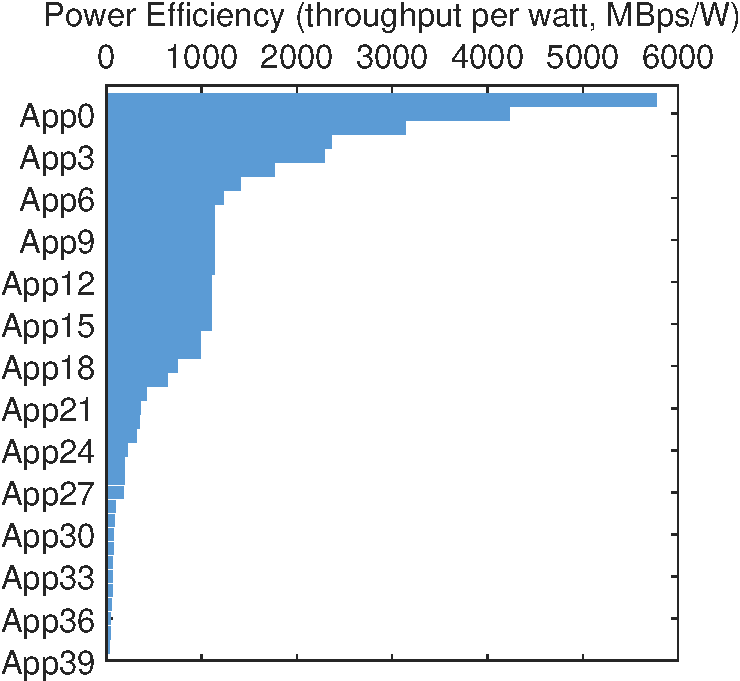
\includegraphics[width=1\textwidth]{fig/effIntro.pdf}
%    \caption{Platform \newtext{Efficiency} for Applications}
%	\label{fig:perf}
%  \end{minipage}
%\end{figure}


%In \figref{fig:domainDSE}, many-application DSE has challenges in both design space traversal and a single design point (one platform) evaluation. Due to targeting to multiple applications, the design space of platform allocation is significantly larger than single application design, \newtext{and an efficient traversal is necessary.} 
%Furthermore, the evaluation for many applications needs to have a fair focus on every application and provide an aggregated value to judge design quantitatively. Current platform evaluation primarily focuses the effects of the platform on one application in isolation. When moving to a set of applications, the simple average sum of all application performances is unfair. \figref{fig:perf} demonstrates the challenge of a MAAR platform evaluation. Because of the big variation among different applications' \newtext{efficiency} on the platform, the 10\% highest efficiency applications will dominate the DSE, if the evaluation simply sums all performances. As a result, the designed platform will not be efficient for many \newtext{low-efficiency} applications. To achieve a highly flexible and an efficient MAAR platform, a fair evaluation needs to aid the DSE in balancing the consideration of all applications.



To solve the challenges, this paper introduces Unified ACC-rich Platform Allocation (UPA), guided by a platform evaluation for many applications with a balanced focus. The contributions of this paper are: (1) providing the flow of UPA, which is a combination of a heuristic traverse, elitist genetic algorithm (GA) and a fair evaluation for many applications; (2) defining relative efficiency of an application on a platform to have a normalized measure of improvement/achievement for different applications; (3) evaluating multiple methods to aggregate efficiency of many applications on a platform to quantitatively compare different platforms. 
The UPA fairly considers the contribution of many applications, and produces an efficient platform supporting all applications. 
In experiments using OpenVX applications, UPA's unified platform with 12 ACCs achieves 4.59 times the average efficiency improvement of dedicated platforms (FDP), and 1.41 times the improvement of DSS~\cite{zhang2018ds}, a previous unified platform design with an unfair evaluation. 


This paper is organized as follows: \secref{sec:related} summarizes the related works. \secref{sec:pre} introduces target ACC-rich platform and evaluation model for individual application. \secref{sec:eval} introduces MAAR DSE and fair MAAR platform evaluation methodology. \secref{sec:results} evaluates and analyzes the benefits of MAAR DSE with fair evaluation. Finally \secref{sec:conclusion} concludes this paper.


